\section{Service de Nommage}

    \subsection{Besoin d'un serivce de nommage}

        \begin{enumerate}
            \item Initialiser le bus CORBA : obtenir l’ORB
            \item Initialiser l’adaptateur d’objets : obtenir le POA
            \item Créer les implantations d’objets
            \item Enregistrer les implantations par l’adaptateur
            \item \textbf{Diffuser leurs références (IOR)}
                    \begin{itemize}
                        \item afficher une chaîne codifiant l’IOR ou
                        \item stocker l’IOR dans un fichier
                    \end{itemize}

            \textbf{OU Utiliser un service de nommage}
            \item Attendre des requêtes venant du bus
            \item Destruction du Bus
        \end{enumerate}

    \subsection*{Besoins de nommage et client CORBA}

        \begin{enumerate}
            \item Initialiser le bus (ORB)
            \item Créer les souches des objets à utiliser
                \begin{enumerate}
                    \item obtenir les références d’objet (IOR)
                        \begin{itemize}
                            \item copier/coller l’IOR affichée coté serveur ou
                            \item lire le fichier contenant l’IOR \\
                            \textbf{OU Accéder au service de nommage}
                        \end{itemize}
                    \item convertir vers les types nécessaires (narrow)
                \end{enumerate}
        \end{enumerate}

    \subsection{Les services de nommage : usage}

        Les services de nommage (ex: rmiregistry) sont utilisés :
    \begin{itemize}
        \item Pour stocker des objets
        \item Pour offrir un point d'accès aux applications réparties
        \item Référentiels d'entreprise pour accéder à :
            \begin{itemize}[label= \ding{230}]
                \item des applications (machine/port), 
                \item des bases de données,
                \item des informations de sécurité (gestion des accès au sein d'une entreprise)
                \item des dispositifs tels que les imprimantes
            \end{itemize}
    \end{itemize}

    \subsection{Service de nommage pour CORBA :}
            \begin{center}
                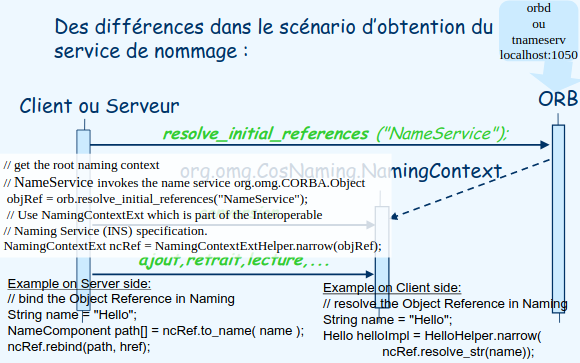
\includegraphics[scale= 0.6]{chap3/corbaname1.png}
            \end{center}


        -----------------% CORBA vs REST----------------

\section{Interopérabilité avec CORBA}
    Objectif = étendre l’interopérabilité entre des ORB différents,voir des systèmes objets “non CORBA”.
    \par Que faut-il pour interopérer ?
    \begin{enumerate}
        \item Manipuler un modèle objet identique.
        \item tre capable d’interpréter convenablement une référence d’objet (ex : localiser son implémentation).
        \item Être capable de véhiculer les invocations et les exceptions.
        \item Manipuler une représentation communes des types, indépendamment des systèmes sous jacent (condition nécessaire dans un environnement constitué d’un seul ORB).
    \end{enumerate}
\vspace*{0.8cm}
\ding{43} \textbf{Solution apportée dans CORBA 2 (CORBA 1 normalise uniquement l’interface de programmation). La version 2 définit :}
\begin{itemize}
    \item Des mécanismes de ponts.
    \item Un protocole standard : \cite{GIOP} , ainsi que sa correspondance sur TCP/IP : IIOP
    \item Des environnements spécifiques (ex : interopérabilité avec DCOM ou par DCE).
\end{itemize}

\ding{42} Compatible CORBA 2 = API CORBA + \cite{IIOP}. 

\begin{flushleft}
\textit{GIOP : Global Inter-ORB Protocol.\\
IIOP : Internet Inter-ORB Protocol}
\end{flushleft}

\paragraph*{Utilisation native de IIOP.}
    \begin{itemize}
        \item Interopérabilité d’office.
        \item Le plus courant dans les ORB commercialisés aujourd’hui.
        \item Permet la mise en œuvre de protocoles optimisés, adaptés à certains types d’environnements ou d’applications.
        \item Conservation de l’existant.
        \item Le pont mémorise des objets proxies
        \item Conversion de protocole, de référence d’objet, voir de modèle objet.
        \item Combinaison de ponts + IIOP en fond de panier.
    \end{itemize}


      
      
\section{CORBA vs REST}

REST n'est pas basé sur les protocoles mais c'est bien un ensemble de principes architecturaux. C'est une architecture
communication point à un point, non fiable contrairement à CORBA. Il ne nécessite pas un outil standard mais un URI standard pour l'échange de 
formation. Il prend en charge JSON, XML et les microformats.La charge peut etre de n'importe quel format tout comme CORBA. Contient un 
gestionnaire d'erreur intégré.

\begin{center}
    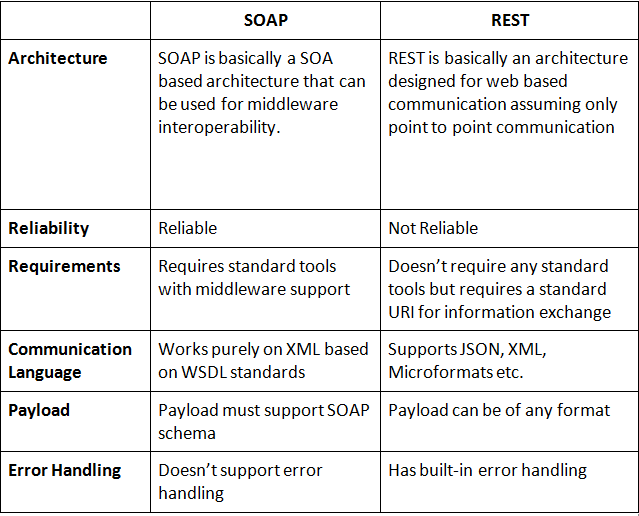
\includegraphics[scale= 0.7]{chap3/resr.png}
\end{center}


\section{CORBA  vs  SOAP}

La technologie middleware CORBA est plus rapide que le protocole de communication standard SOAP lors des échanges, et ce à cause du nombre d'informations qu'impose le format XML sur lequel est bâti SOAP,

Par contre lorsque le volume de données transmis par SOAP est faible par rapport au volume total de données échangés ce n'est plus un handicap.